\section{TWMM efficiency}
\subsection{Comparing with CF-AMM}
For a CF-AMM with the invariant function $x \cdot y = L$, the amount of output asset $\Delta y$ received for a given input amount $\Delta x$ is calculated based on the initial reserves of the assets.

The formula, which accounts for a standard percentage trading fee, is:

\begin{equation}
	\label{eq:cfamm_price_function}
	\Delta y=\frac{ 
		\begin{aligned} 
			\Delta x\cdot997\cdot R_{in}\cdot m \cdot\frac{P_{in}}{P_{out}} 
		\end{aligned}
	}{
		\begin{aligned} 
			R_{in}\cdot m \cdot1000+ \Delta x\ \cdot997\cdot\sqrt{\frac{P_{in}}{P_{out}}}
		\end{aligned}
	}
\end{equation}

To provide a clear performance benchmark, we will utilize a standard CF-AMM formula. This formula calculates the output asset amount for a given input amount, including a 0.3\% fee charged on the input. To facilitate a direct comparison, the CF-AMM model is parameterized using prices ($P_{in}, P_{out}$) and a liquidity level derived from the input asset's reserve ($R_{in}$), mirroring the variables used in the TWMM's swap invariant.

We will now compare the trade execution of this CF-AMM against the TWMM across several key scenarios. These include conditions with varying cashback reserves, near-zero deviation, and significant initial deviation.

In the following charts, the performance is illustrated as follows:
\begin{itemize}
	\item The \textbf{red line} represents the \textbf{TWMM}.
	\item The solid \textbf{blue line} represents the standard \textbf{CF-AMM} ($m=1$).
	\item The dashed \textbf{blue line} represents a \textbf{CF-AMM with tenfold liquidity}, providing a benchmark for capital efficiency ($m=10$).
\item The \textbf{Blue Zone} highlights a fundamental constraint of the TWMM: the output amount cannot exceed the total available reserve of the output asset ($\Delta Q_{out} \leq R_{out}$).
\end{itemize}
\begin{figure}[h!]
	\centering
	\begin{subfigure}{0.4\textwidth} % Adjust width as needed
		\centering
		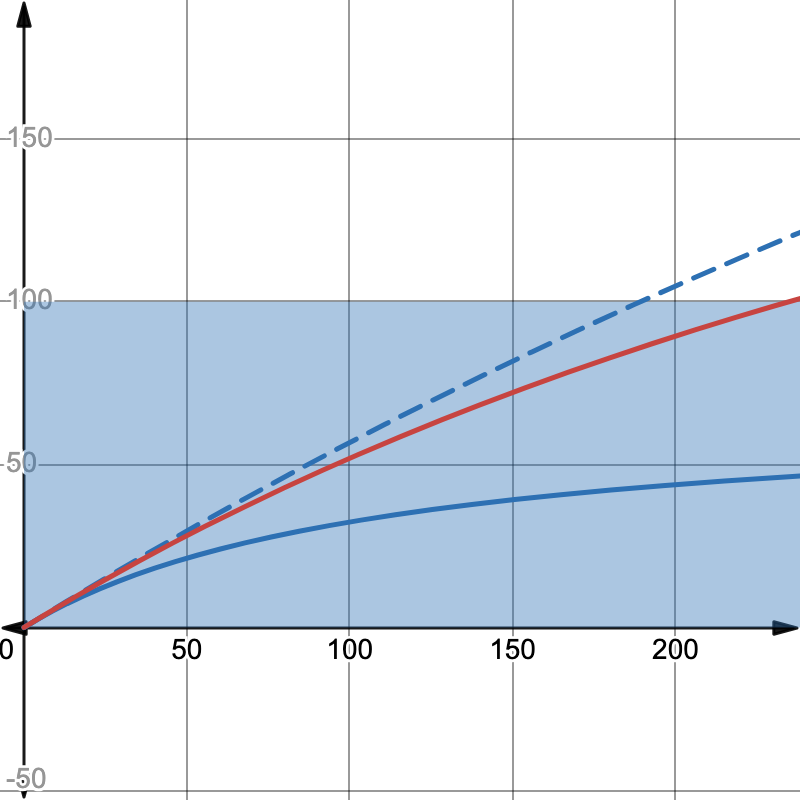
\includegraphics[width=\linewidth]{comparing_with_cfamm_deviation_big.png} % Adjust width/height
		\caption{Deviation hight on both assets}
		\label{fig:img4}
	\end{subfigure}
	\hfill % Adds horizontal space between images
	\begin{subfigure}{0.4\textwidth}
		\centering
		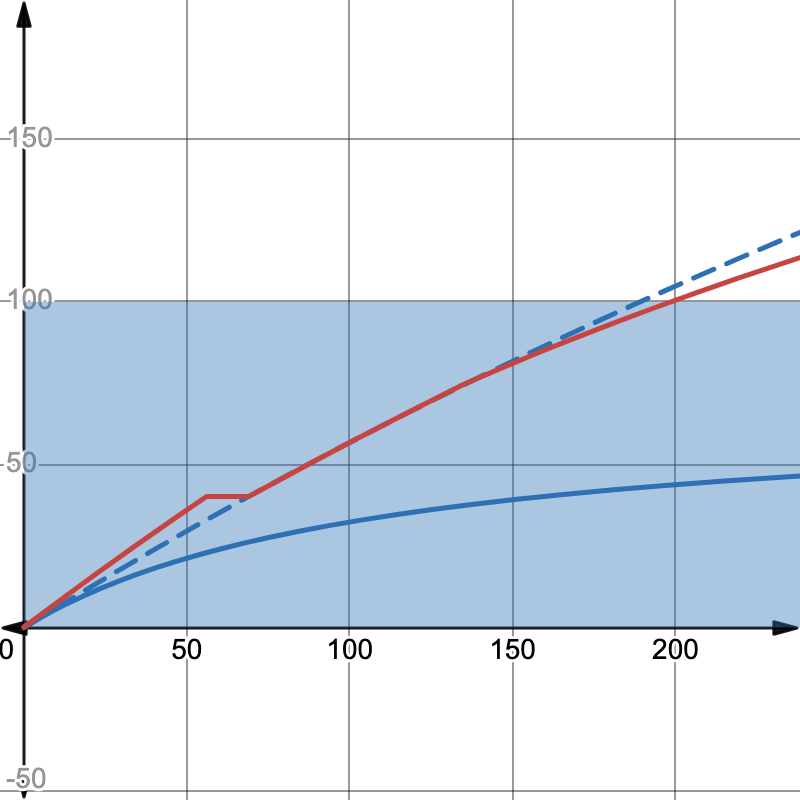
\includegraphics[width=\linewidth]{comparing_with_cfamm_deviation_one_asset.png} % Adjust width/height
		\caption{Cashback on one asset}
		\label{fig:img5}
	\end{subfigure}
	\caption{Comparison in deviation cases}
	\label{fig:img6}
\end{figure}
\FloatBarrier
\begin{figure}[h!]
	\centering
	\begin{subfigure}{0.4\textwidth} % Adjust width as needed
		\centering
		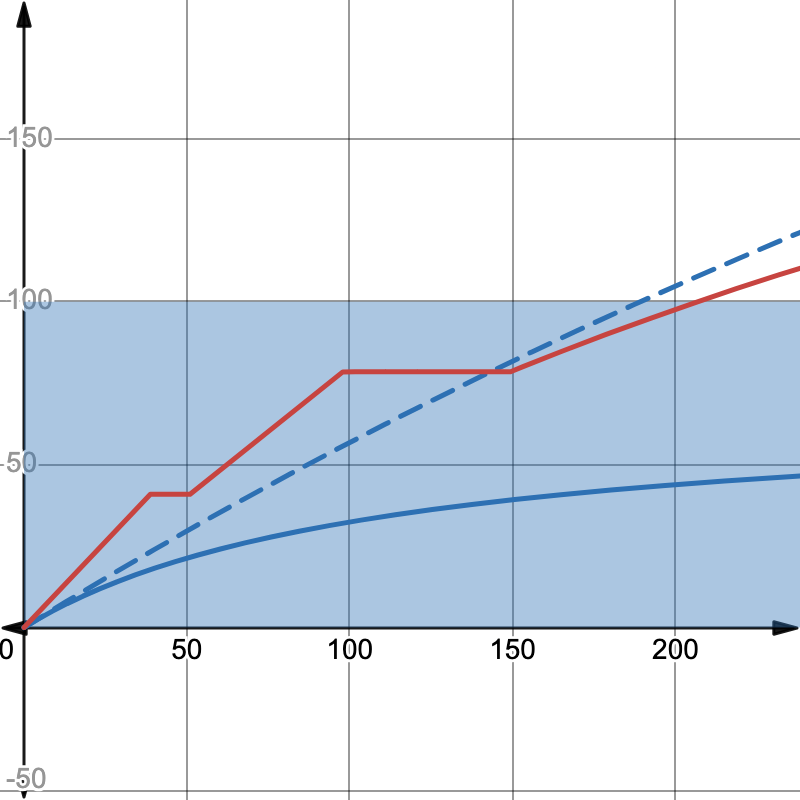
\includegraphics[width=\linewidth]{comparing_with_cfamm_no_deviation_big_cashback.png} % Adjust width/height
		\caption{Cashback on both assets}
		\label{fig:img7}
	\end{subfigure}
	\hfill % Adds horizontal space between images
	\begin{subfigure}{0.4\textwidth}
		\centering
		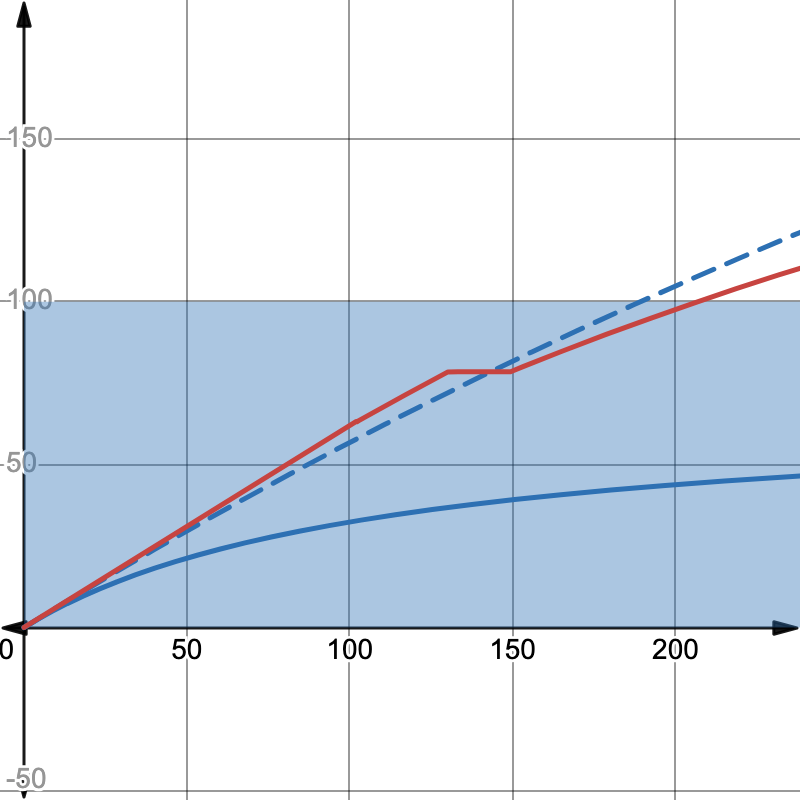
\includegraphics[width=\linewidth]{comparing_with_cfamm_no_deviation_no_cashback.png} % Adjust width/height
		\caption{No cashbacks}
		\label{fig:img8}
	\end{subfigure}
	\caption{Comparison in non deviation cases}
	\label{fig:img9}
\end{figure}
\FloatBarrier

The analysis demonstrates that the TWMM offers superior capital efficiency across a wide range of trading scenarios. Excluding cases of extreme deviation—where the pool holds a severe surplus or deficit of an asset—the TWMM's performance is comparable to that of a standard CF-AMM with as much as tenfold its TVL. This finding and ability to put multiple trading pairs into one TWMM pool indicates a profound improvement in capital utilization, allowing the TWMM to facilitate large trades with significantly less liquidity than traditional models.

\subsection{Impermanent Loss Mitigation}

In the context of CF-AMMs, impermanent loss represents the opportunity cost a liquidity provider incurs compared to simply holding the assets in their wallet. While the TWMM does not eliminate this risk, it provides powerful tools to actively manage and mitigate it by reframing liquidity provision as a form of active portfolio management.

The key to this mitigation lies in the ability to dynamically adjust the target weights of the assets within the pool. This flexibility enables several strategic possibilities that are unavailable in static CF-AMMs:
\begin{itemize}
	\item \textbf{Fee Optimization:} A pool manager can increase the target share of assets anticipated to have high trading volume. This strategy aims to maximize fee generation, which can serve as a direct offset against potential impermanent loss.
	
	\item \textbf{Exposure and Risk Management:} Conversely, a manager can reduce the target share of a highly volatile asset. This allows the pool to maintain exposure to the asset's potential upside while minimizing the magnitude of impermanent loss caused by its price fluctuations.
\end{itemize}

Consequently, the TWMM LP token transcends its role as a simple claim on pooled assets. It becomes a tokenized representation of a managed financial strategy. While this strategy may not outperform every individual asset in the portfolio, it can be calibrated to offer a superior risk-adjusted return profile, effectively serving as a more stable store of value compared to a passive holding strategy.